\documentclass{article}

\usepackage{hyperref}
\usepackage{graphicx}
\usepackage{multirow}
\usepackage{subfig}
\usepackage{float}
\usepackage{longtable}
%\usepackage{blindtext}

\graphicspath{{./fig/}}

\begin{document}


\title{Physically Based Sound\\CIS 563}
\date{May 4, 2012}
\author{Jiali Sheng and Jordan Brindza}
\maketitle
  

\section{Introduction}
For this project, we plan to physically generate sound for rigid body
collisions. To simulate sound, we followed the implementation of the paper
"Interactive Sound Synthesis for Large Scale Enviromenets" \cite{Raghuvanshi}. First, we
reconstructed the objects in the scene as massspring systems, and calculated
the Gain matrix , and other coefficients as according to the paper. During
run-time, we apply the force onto our mass-spring system to generate multiple
signals that sum up to a sound wave. 

\section{Sound Modeling}
The main equations we implemented are as follows:

  % equations
  $$
    % system model ODE
    M\frac{d^2 r}{dt^2} + (\gamma M + \eta K) \frac{dr}{dt} + Kr = f
  $$

  $$
    % diagonalized K
    K = GDG^{-1}
  $$

  $$
    % substituting for K
    \begin{array}{ccc}
      M\frac{d^2 r}{dt^2} + (\gamma M + \eta GDG^{-1}) \frac{dr}{dt} + GDG^{-1}r & = & f \\[11pt]
      G^{-1} M\frac{d^2 r}{dt^2} + (\gamma G^{-1} M + \eta DG^{-1}) \frac{dr}{dt} + DG^{-1}r & = & G^{-1} f \\[11pt]
      \textrm{$M$ is diagonal so } G^{-1}M = MG^{-1} & & \\[11pt]
      M G^{-1} \frac{d^2 r}{dt^2} + (\gamma M + \eta D)G^{-1} \frac{dr}{dt} + DG^{-1}r & = & G^{-1} f \\[11pt]
      \textrm{Using change of variables let } z = G^{-1} r & & \\[11pt]
      M \frac{d^2 z}{dt^2} + (\gamma M + \eta D) \frac{dz}{dt} + Dz & = & G^{-1} f \\[11pt]
    \end{array}
  $$

  $M$ and $D$ are both diagonal martices resulting in a set of $3n$ independent differential equations for each $z_i$. 
These equations are derivid from force calculations of the system.

  $$
    % ode solution for damped oscillator 
    \begin{array}{ccc}
      z_{i}(t) & = & c_{i} e^{w_{i}^{+}t} + \bar{c}_{i} e^{w_{i}^{-}t} \\ 
      w_{i}^{\pm} & = & \frac{-(\gamma \lambda_{i} + \eta) \pm \sqrt{(\gamma \lambda_{i} + \eta)^2 - 4 \lambda_{i}}}{2}
    \end{array}
  $$
where lambda is the eigen values of the K-matrix. And gamma and eta are enviorment and material damping constants. 
  $$
    % derivative of z_i
    v_{i} = \frac{dz_{i}}{dt} = c_{i} w_{i}^{+} e^{w_{i}^{+}t} + \bar{c}_{i} w_{i}^{-} e^{w_{i}^{-}t}  
  $$

  $$
    % constants update from impulse
    c_{i} \gets c_{i} + \frac{g_{i}}{m_{i} (w_{i}^{+} - w_{i}^{-}) e^{w_{i}^{+} t_{0}}}
  $$


\section{Performance}

We first looked at our input data. Our input is an xml file with information on how to generate a few supported primitives. With these primatives, we generated a mass-spring system based on our guess of how a mesh of the same primative would look like. Figure 1 shows a simple example of a cube primative. We store the data in an adjacency list. 

  \begin{figure}[H]
    \begin{center}
      \includegraphics[width=0.8\columnwidth]{cube_mesh_mesh_plot}
    \end{center} 
    \caption{Simple, example mesh for a cube with partices at each corner.}
  \end{figure}

Given our mass-spring system in the adjacency list, we then have to calcualte the elastic force matrix (we'll call it the k-matrix). We assumed that all the springs in the mass-spring-system have the same k-constant. By Young's Modulus Theorem, this means we can factor the k-constant out when we first calculate the matrix. This K-matrix is a square matrix of size 3*N by 3*N -- N is the number of masses in the system. For the K-matrix, for each spring (from mass i to mass j), we will do +1 on cells  (i,i) and (j,j), and -1 on cells (i,j), and (j,i), this is repeated for 2*N and 3*N. Figure 2 shows a visualization of our K-matrix for the cube. 

  \begin{figure}[H]
    \begin{center}
        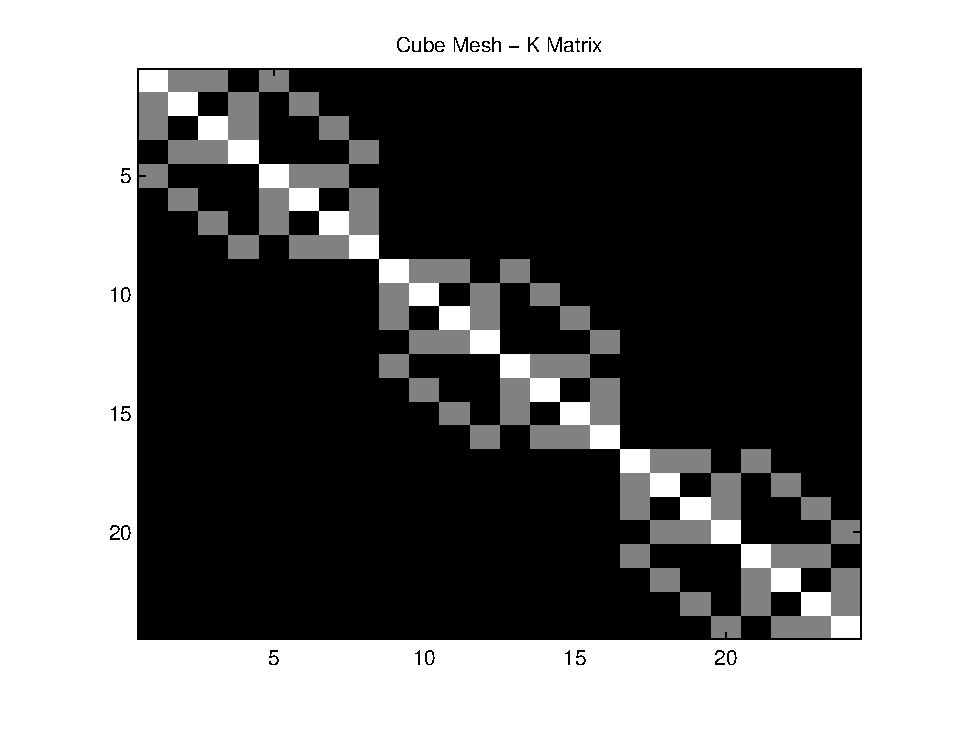
\includegraphics[width=0.8\columnwidth]{cube_mesh_Kmatrix} 
    \end{center} 
    \caption{Visualization of the full K matrix for the simple cube mesh. The
              black cells are $0$, the gray cells have the value $-k$ and the white
              cells have the value $+2k$.}
  \end{figure}

Everytime a collision is detected, our calculations will take the impulse force at the point of contact, and simulate the force on the mass-spring system. The result is a series of signals produced by each spring in the system. To obtain the sound sample, we sum over the different signals and output it as a buffer array into the FMOD sound package. Based on sampling ratios, and theories of perceptions, we can adjust the sampling rate and cut out inaudiable signals to cut down computing time. Figure three shows graphs of the signals produced by striking the cube and sampling at different rates. 

  \begin{figure}[H]
    \begin{center}$
      \begin{tabular}{cc}
        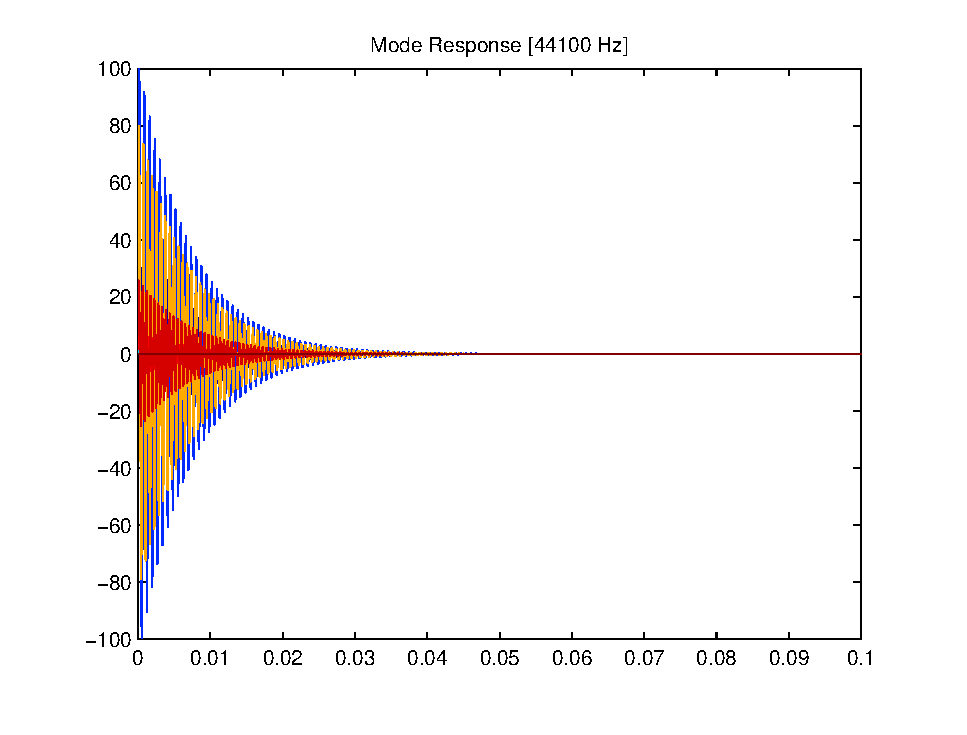
\includegraphics[width=0.5\columnwidth]{cube_mode_resp_44100hz}
        &
        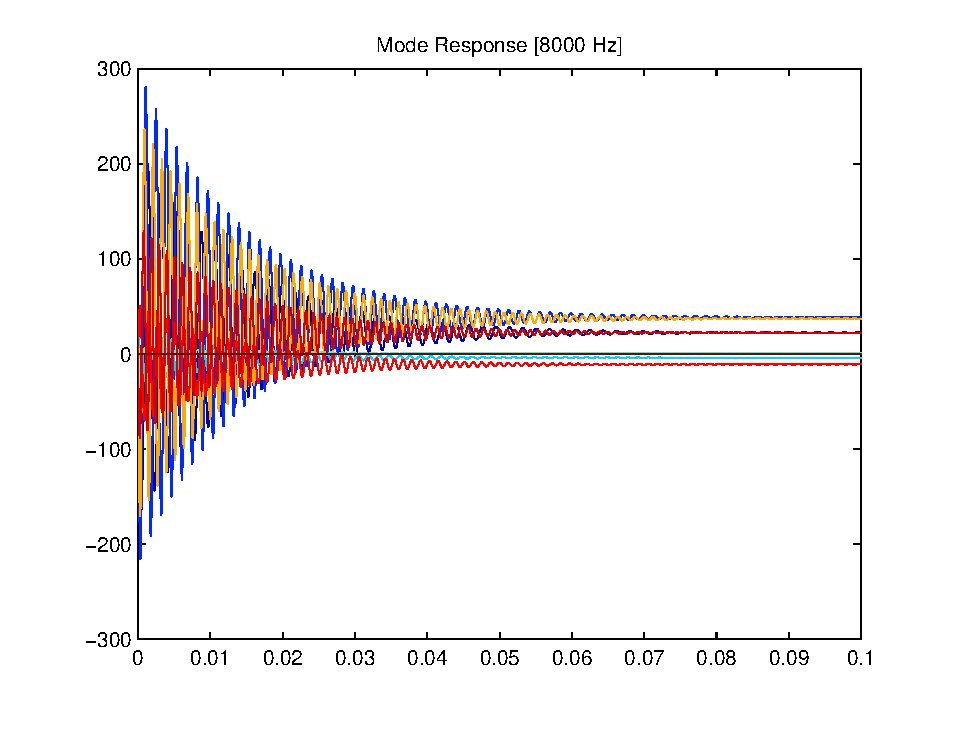
\includegraphics[width=0.5\columnwidth]{cube_mode_resp_8000hz} 
      \\
        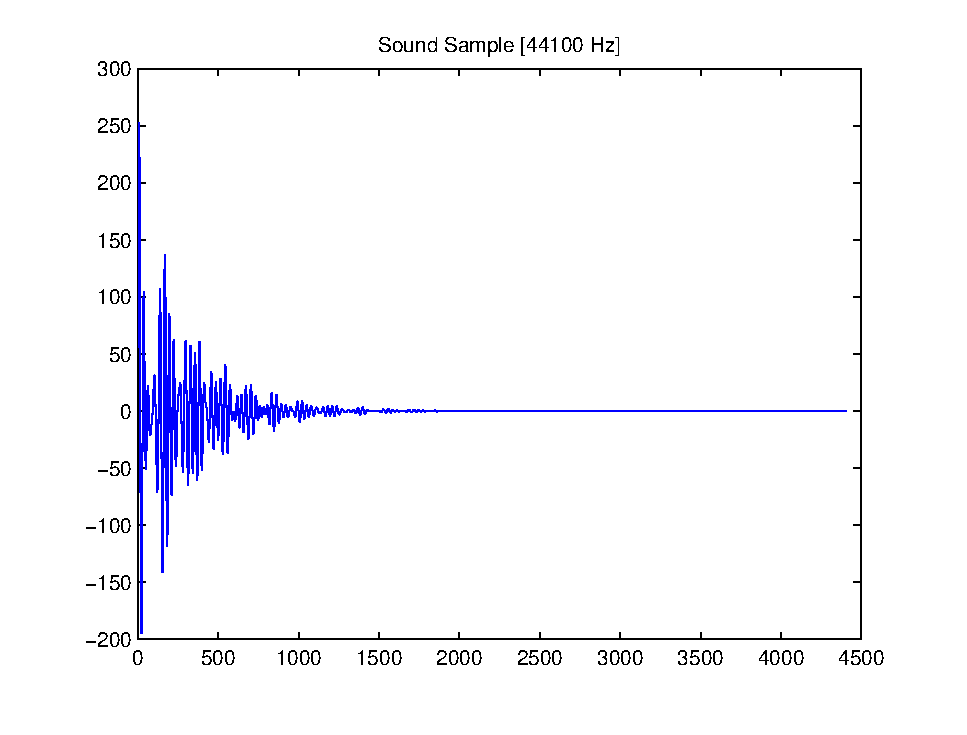
\includegraphics[width=0.5\columnwidth]{sound_sample_44100hz}
        &
        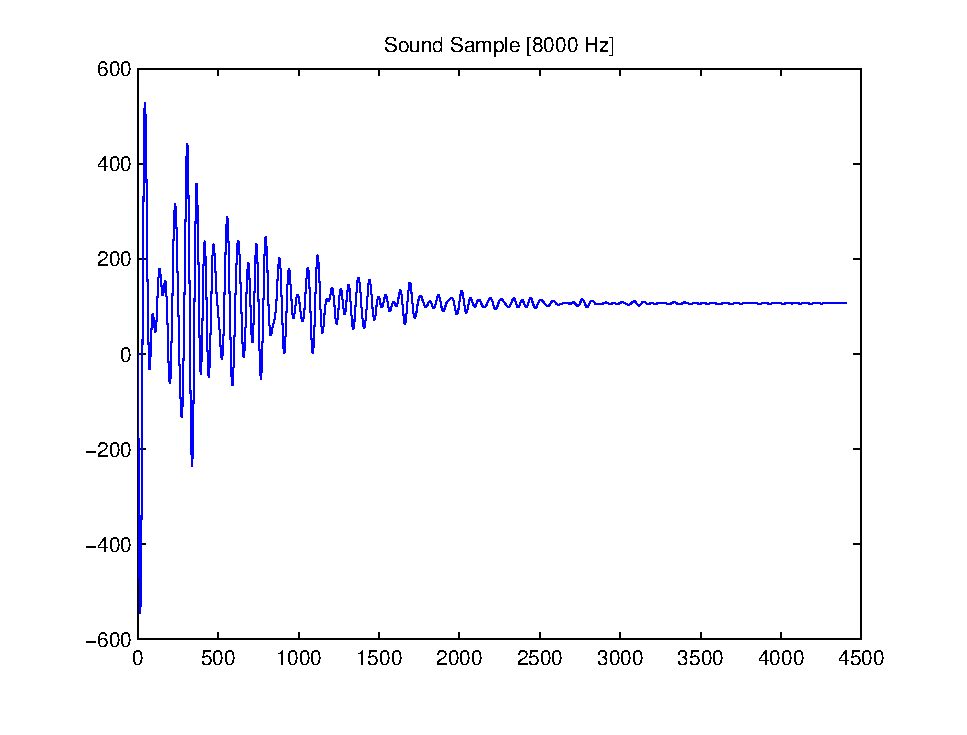
\includegraphics[width=0.5\columnwidth]{sound_sample_8000hz}
      \end{tabular}$
    \end{center}
    \caption{Plots of synthesized sound for a unit impluse on one of the cube
              vertices. The top row shows the individual mode responses (left was created
              at 44.1 kHz and the right at 8 kHz). The bottom row is the final sound
              sample of the summed mode responses (the left was sampled at 44100
              kHz and the right at 8 kHz).}
  \end{figure}

\section{Results}


  % table example
  %\begin{center}
  %  \begin{tabular}{|c|c|c|c|}
  %    \hline
  %    Environment & Completion Time [s] & Max Position Error [m] & Max Orientation Error \\
  %    \hline
  %    1         & $85.40 $ &  $0.5220$ & $1.9745$ \\
  %    1         & $85.72 $ &  $0.3895$ & $0.1701$ \\
  %    7         & $120.52$ &  $0.9430$ & $0.5883$ \\
  %    7.2       & $120.82$ &  $1.2152$ & $1.9514$ \\
  %    \hline
  %  \end{tabular}
  %  \label{tab:myfirsttable}
  %\end{center}

  % grouped images example
  %\begin{figure}[H]
  %  \begin{center}$
  %    \begin{tabular}{cc}
  %      \includegraphics[width=0.5\columnwidth]{block_match_left_rgb}
  %      &
  %      \includegraphics[width=0.5\columnwidth]{block_match_left_block_seg} 
  %    \end{tabular}$
  %  \end{center}
  %  \caption{Example RGB image (left) and segmented regions (right).}
  %\end{figure}

  % single image example
  %\begin{figure}[H]
  %  \begin{center}
  %    \includegraphics[width=0.8\columnwidth]{block_match_stereo_corr}
  %  \end{center} 
  %  \caption{Example stereo correspondence.}
  %\end{figure}


%\bibliography{report} \bibliographystyle{plain}

\end{document}

